\documentclass[aspectratio=169]{beamer}

% ------------------ Tema ------------------
\usetheme{Madrid}
\usecolortheme{default}
\setbeamertemplate{navigation symbols}{}

% ------------------ Paketler ------------------
\usepackage[utf8]{inputenc}
\usepackage[T1]{fontenc}
\usepackage[turkish]{babel}
\usepackage{lmodern}
\usepackage{graphicx}
\usepackage{booktabs}
\usepackage{array}
\usepackage{tikz}
\usetikzlibrary{positioning,arrows.meta,shapes.geometric}

\graphicspath{{../figures/}{figures/}}

% ------------------ Başlık Bilgileri ------------------
\title{Banka Pazarlama Kampanyalarında Müşteri Tahmin ve Açıklanabilirlik Sistemi}
\subtitle{BLM308 Veri Madenciliği -- Final Proje}
\author{Sude ANLAŞ \and Doğan Fatih OĞUR \and Merve Naz ORAN}
\institute{Gedik Üniversitesi -- Bilgisayar Mühendisliği}
\date{Bahar 2026}

\begin{document}

%------------------------------------------------
\begin{frame}
    \titlepage
\end{frame}

%------------------------------------------------
\begin{frame}{İçerik}
    \tableofcontents
\end{frame}

%================================================
\section{Giriş}
%================================================

\begin{frame}{Problem Tanımı}
    \begin{block}{Temel problem}
        Banka, pazarlama kampanyasında hangi müşterilerin vadeli mevduata abone olma ihtimalinin yüksek olduğunu önceden tahmin etmek istemektedir.
    \end{block}

    \begin{itemize}
        \item Rastgele arama stratejisi zaman ve maliyet kaybı oluşturabilir.
        \item Sınırlı çağrı merkezi kapasitesi daha verimli kullanılmalıdır.
        \item Model yalnızca tahmin üretmemeli; karar gerekçesini de açıklamalıdır.
    \end{itemize}
\end{frame}

\begin{frame}{Motivasyon ve İş Değeri}
    \begin{columns}[T]
        \column{0.50\textwidth}
        \textbf{İş değeri}
        \begin{itemize}
            \item Yüksek potansiyelli müşterilere öncelik verme
            \item Kampanya dönüşüm oranını artırma
            \item Gereksiz aramaları azaltma
        \end{itemize}

        \column{0.50\textwidth}
        \textbf{Açıklanabilirlik ihtiyacı}
        \begin{itemize}
            \item Bankacılıkta kararın gerekçesi önemlidir.
            \item Kara kutu model önerisi denetlenebilir olmalıdır.
            \item Pazarlama ekibi modeli iş bağlamında yorumlayabilmelidir.
        \end{itemize}
    \end{columns}
\end{frame}

\begin{frame}{Proje Farkı}
    \begin{itemize}
        \item Yalnızca sınıflandırma modeli kurulmadı; uçtan uca CRISP-DM süreci izlendi.
        \item Random Forest ve Çok Katmanlı Algılayıcı kara kutu model olarak karşılaştırıldı.
        \item Görüşme süresi değişkeni için veri sızıntısı analizi yapıldı.
        \item Model sonuçları McNemar testiyle istatistiksel olarak karşılaştırıldı.
        \item Türkçe bir tahmin ve açıklanabilirlik arayüzü hazırlandı.
    \end{itemize}
\end{frame}

%================================================
\section{Yöntem}
%================================================

\begin{frame}{Genel Akış: CRISP-DM}
    \centering
    \begin{tikzpicture}[
        node distance=1.0cm and 0.65cm,
        every node/.style={draw, rectangle, rounded corners, align=center,
            minimum height=0.85cm, minimum width=2.0cm, font=\small}
    ]
        \node (is) {İş\\Anlayışı};
        \node (veri) [right=of is] {Veri\\Anlayışı};
        \node (haz) [right=of veri] {Veri\\Hazırlığı};
        \node (model) [right=of haz] {Model\\Eğitimi};
        \node (deg) [right=of model] {Değer-\\lendirme};
        \node (xai) [right=of deg] {XAI ve\\Arayüz};

        \draw[-Latex] (is) -- (veri);
        \draw[-Latex] (veri) -- (haz);
        \draw[-Latex] (haz) -- (model);
        \draw[-Latex] (model) -- (deg);
        \draw[-Latex] (deg) -- (xai);
        \draw[-Latex, dashed] (deg.south) to[out=-90, in=-90] (haz.south);
    \end{tikzpicture}

    \vspace{0.4cm}
    \small Modelleme çıktıları yalnızca metrik olarak değil, iş değeri ve açıklanabilirlik açısından da yorumlandı.
\end{frame}

\begin{frame}{Kullanılan Araçlar}
    \begin{columns}[T]
        \column{0.48\textwidth}
        \textbf{Modelleme ve analiz}
        \begin{itemize}
            \item Python
            \item pandas, numpy
            \item scikit-learn
            \item matplotlib, seaborn
        \end{itemize}

        \column{0.48\textwidth}
        \textbf{Açıklanabilirlik ve sunum}
        \begin{itemize}
            \item SHAP / LIME yaklaşımı
            \item Streamlit arayüzü
            \item Beamer sunum
            \item Word raporu
        \end{itemize}
    \end{columns}
\end{frame}

%================================================
\section{Veri}
%================================================

\begin{frame}{Veri Kaynağı ve Tanım}
    \begin{itemize}
        \item \textbf{Kaynak:} UCI Bank Marketing veri seti
        \item \textbf{Örnek sayısı:} 41.188
        \item \textbf{Girdi değişkeni sayısı:} 20
        \item \textbf{Hedef değişken:} Vadeli mevduata abone olma durumu
    \end{itemize}

    \begin{block}{Sınıf dağılımı}
        Abone oldu: 4.640 \quad (\%11,3) \hfill
        Abone olmadı: 36.548 \quad (\%88,7)
    \end{block}

    \small Bu dağılım nedeniyle yalnızca doğruluk metriğine bakmak yeterli değildir.
\end{frame}

\begin{frame}{Hedef Değişken Dağılımı}
    \centering
    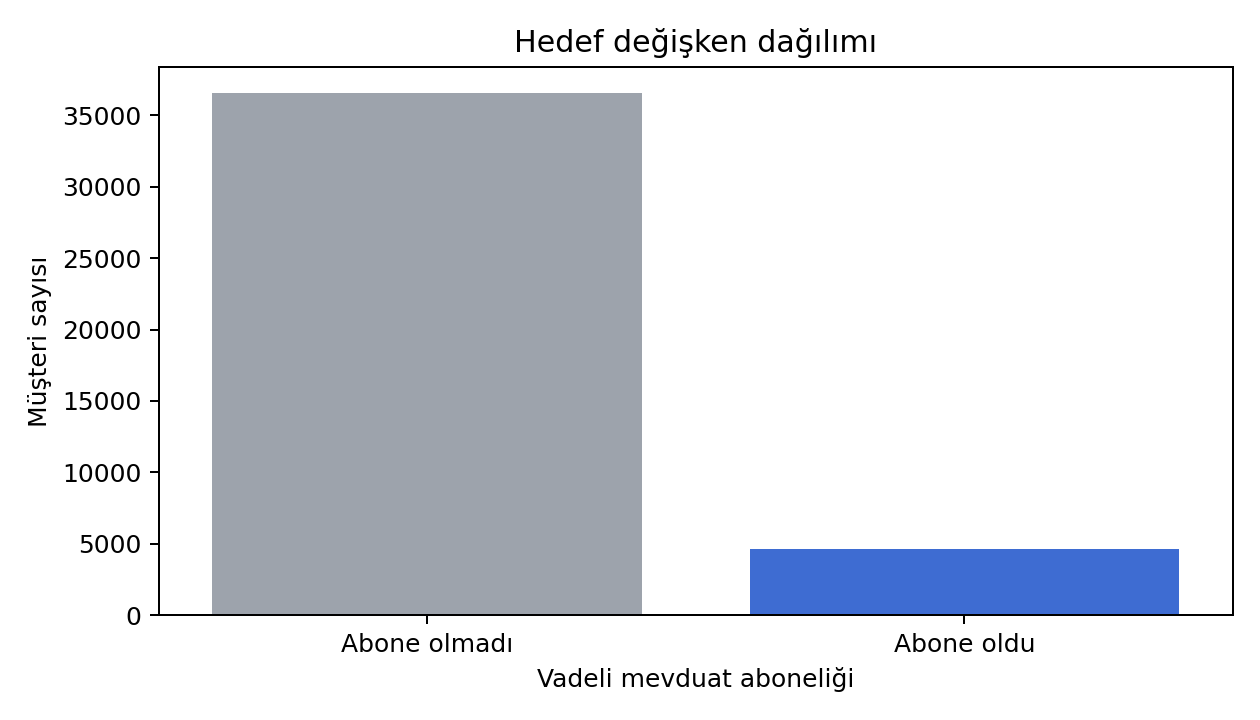
\includegraphics[width=0.72\textwidth]{target_distribution_turkce.png}

    \vspace{0.2cm}
    \small Veri dengesizdir; bu yüzden kesinlik, duyarlılık, F1 ve ROC-AUC birlikte değerlendirilmiştir.
\end{frame}

\begin{frame}{Veri Hazırlığı ve Kritik Karar}
    \begin{enumerate}
        \item Kategorik değişkenler one-hot encoding ile sayısallaştırıldı.
        \item Sayısal değişkenler standartlaştırıldı.
        \item Veri eğitim/test olarak ayrıldı.
        \item Sınıf dengesizliği için class-weight kullanıldı.
    \end{enumerate}

    \begin{alertblock}{Veri sızıntısı farkındalığı}
        Görüşme süresi değişkeni müşteri aranmadan önce bilinmez. Bu nedenle gerçekçi kullanımda modelden çıkarılmıştır.
    \end{alertblock}
\end{frame}

%================================================
\section{Modelleme}
%================================================

\begin{frame}{Seçilen Modeller}
    \centering
    \small
    \begin{tabular}{lll}
        \toprule
        \textbf{Model} & \textbf{Tür} & \textbf{Projedeki Rolü} \\
        \midrule
        Lojistik Regresyon & Temel model & Yorumlanabilir karşılaştırma \\
        Karar Ağacı & Ağaç tabanlı & Kural benzeri referans \\
        Random Forest & Ensemble kara kutu & Ana tahmin modeli \\
        Çok Katmanlı Algılayıcı & Sinir ağı & Alternatif kara kutu model \\
        \bottomrule
    \end{tabular}

    \vspace{0.35cm}
    \small Random Forest, performans ve açıklanabilirlik dengesinden dolayı arayüzde kullanılan ana modeldir.
\end{frame}

\begin{frame}{Deney Kurulumu}
    \begin{itemize}
        \item \textbf{Veri bölme:} \%75 eğitim, \%25 test
        \item \textbf{Bölme yöntemi:} Stratified split
        \item \textbf{Ana metrikler:} Doğruluk, kesinlik, duyarlılık, F1, ROC-AUC
        \item \textbf{Ek değerlendirme:} McNemar testi
        \item \textbf{Uygulama senaryosu:} Görüşme süresi hariç Random Forest
    \end{itemize}
\end{frame}

%================================================
\section{Sonuçlar}
%================================================

\begin{frame}{Performans Karşılaştırması}
    \centering
    \scriptsize
    \begin{tabular}{llrrrrr}
        \toprule
        \textbf{Senaryo} & \textbf{Model} & \textbf{Doğ.} & \textbf{Kes.} & \textbf{Duy.} & \textbf{F1} & \textbf{AUC} \\
        \midrule
        Görüşme süresi dahil & Random Forest & 0.868 & 0.457 & 0.925 & 0.611 & \textbf{0.949} \\
        Görüşme süresi dahil & Çok Katmanlı Algılayıcı & 0.915 & 0.650 & 0.528 & 0.582 & 0.947 \\
        Görüşme süresi hariç & Lojistik Regresyon & 0.835 & 0.367 & 0.644 & 0.467 & 0.805 \\
        Görüşme süresi hariç & Random Forest & 0.864 & 0.430 & 0.633 & \textbf{0.512} & \textbf{0.816} \\
        Görüşme süresi hariç & Çok Katmanlı Algılayıcı & 0.900 & 0.647 & 0.245 & 0.355 & 0.808 \\
        \bottomrule
    \end{tabular}

    \vspace{0.35cm}
    \small Gerçekçi kullanımda görüşme süresi hariç sonuçlar esas alınmıştır.
\end{frame}

\begin{frame}{ROC-AUC Karşılaştırması}
    \centering
    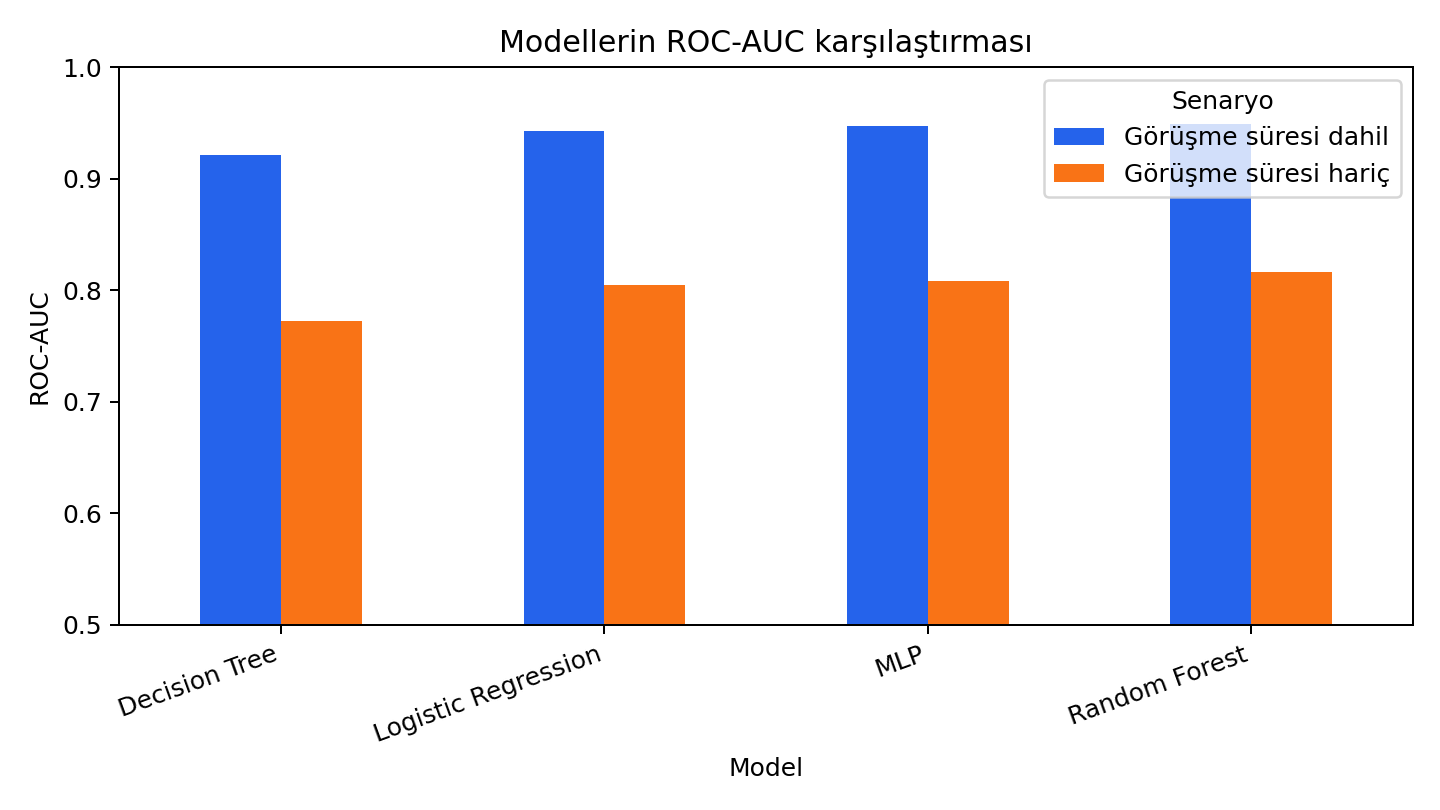
\includegraphics[width=0.76\textwidth]{model_auc_comparison_turkce.png}

    \vspace{0.2cm}
    \small Görüşme süresi dahil senaryo performansı yükseltir; ancak gerçek kampanya öncesi kullanım için yanıltıcı olabilir.
\end{frame}

\begin{frame}{Hata Matrisi: Random Forest}
    \centering
    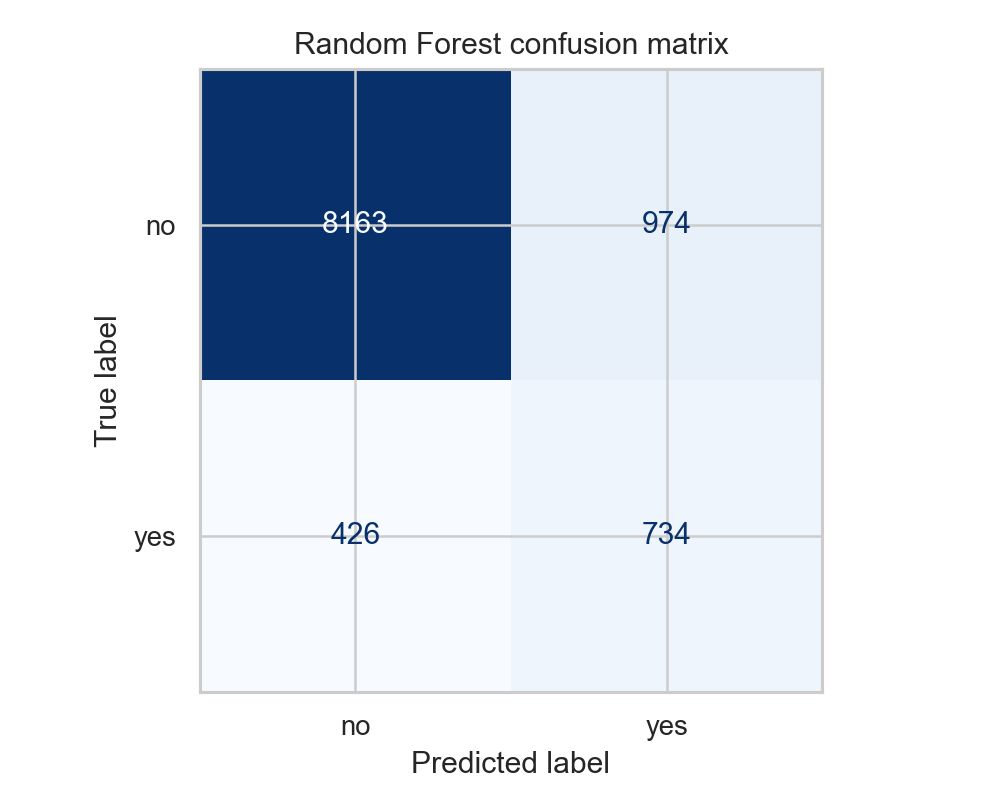
\includegraphics[width=0.48\textwidth]{rf_confusion_matrix.png}

    \vspace{0.2cm}
    \small Model abone olmayan sınıfta güçlüdür; abone olabilecek müşterileri kaçırmamak için duyarlılık ayrıca izlenmelidir.
\end{frame}

\begin{frame}{İstatistiksel Karşılaştırma}
    \begin{block}{McNemar testi: Random Forest vs Çok Katmanlı Algılayıcı}
        \centering
        $b = 450$ \qquad $c = 819$ \qquad $\chi^2 = 106.717$ \qquad $p < 0.001$
    \end{block}

    \begin{itemize}
        \item İki model aynı test örnekleri üzerinde karşılaştırıldı.
        \item p-değeri çok düşük olduğu için hata örüntüleri istatistiksel olarak farklıdır.
        \item Bu sonuç, değerlendirmeyi yalnızca metrik tablosuna bağlı bırakmamıştır.
    \end{itemize}
\end{frame}

%================================================
\section{Açıklanabilirlik}
%================================================

\begin{frame}{Modelin Genel Kararlarını Etkileyen Faktörler}
    \centering
    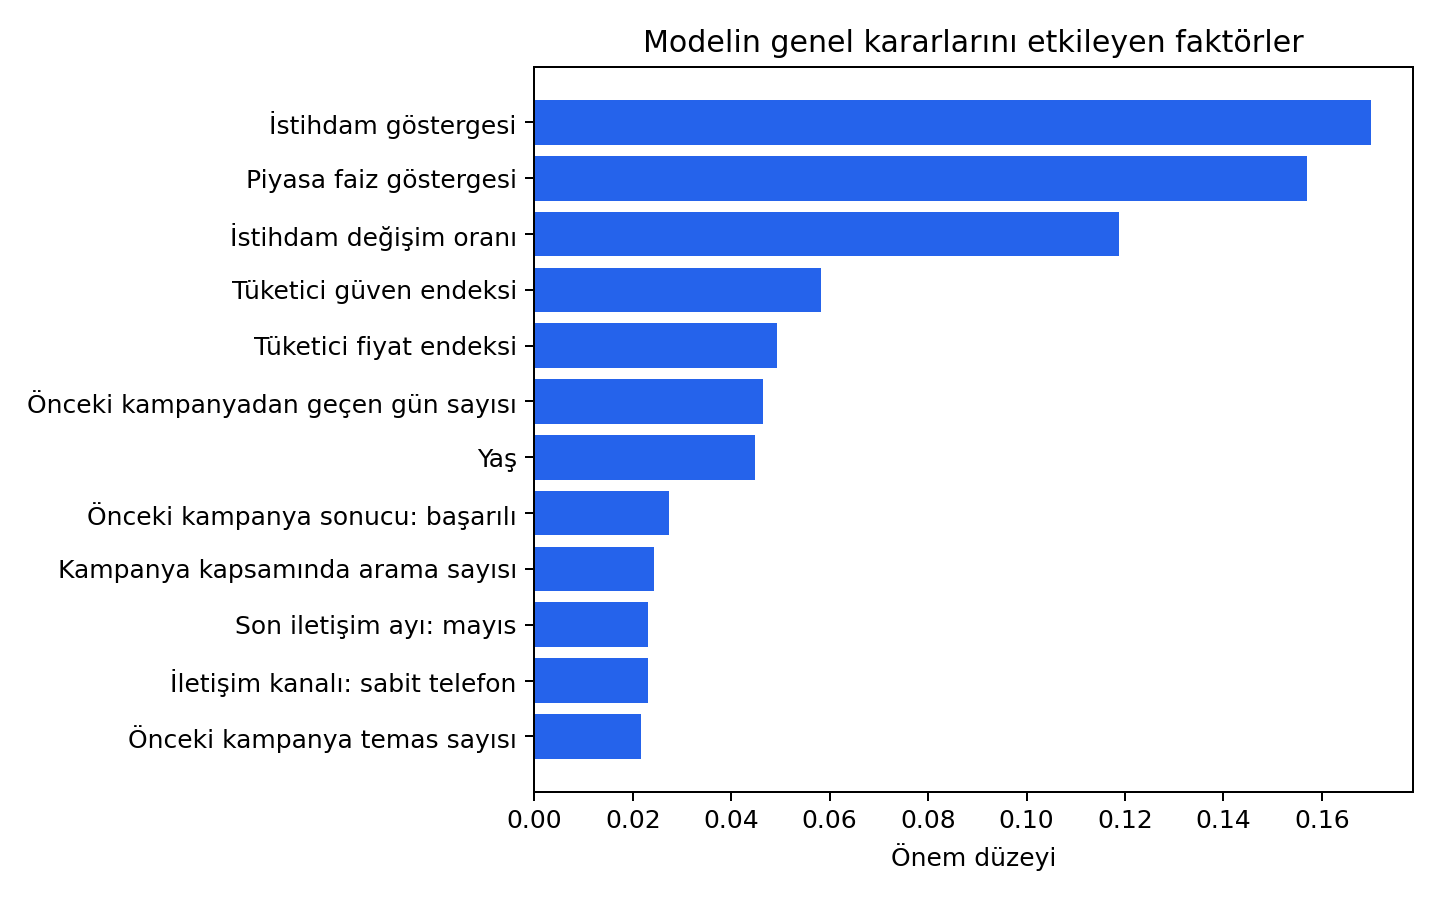
\includegraphics[width=0.82\textwidth]{rf_feature_importance_from_explain.png}

    \vspace{0.2cm}
    \small Ekonomik göstergeler, önceki kampanya sonucu ve kampanya temas bilgileri model kararlarında öne çıkmaktadır.
\end{frame}

\begin{frame}{Tek Müşteri İçin Yerel Açıklama}
    \centering
    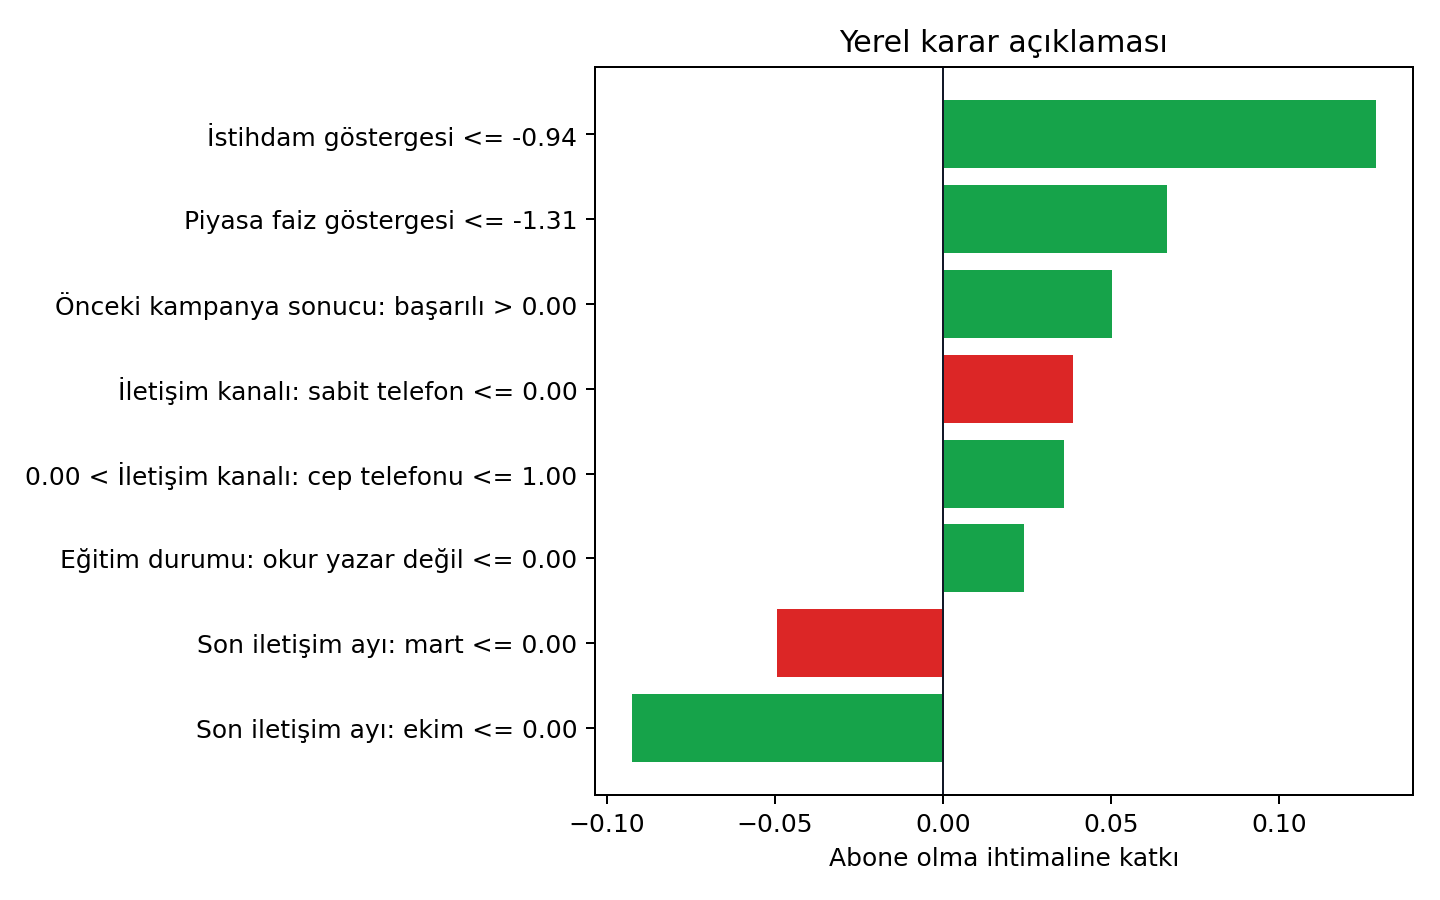
\includegraphics[width=0.82\textwidth]{lime_explanation_from_explain.png}

    \vspace{0.2cm}
    \small Yerel açıklama, belirli bir müşteri için hangi faktörlerin abone olma ihtimalini artırıp azalttığını gösterir.
\end{frame}

\begin{frame}{Açıklanabilirlik Neden Önemli?}
    \begin{itemize}
        \item Kara kutu model kararları daha denetlenebilir hale gelir.
        \item Pazarlama uzmanı modelin önerisini iş bağlamında yorumlayabilir.
        \item Finans alanında güven, şeffaflık ve hesap verebilirlik artar.
        \item Model, yalnızca skor üreten bir araç değil, karar destek sistemi haline gelir.
    \end{itemize}
\end{frame}

%================================================
\section{Uygulama ve Sonuç}
%================================================

\begin{frame}{Türkçe Tahmin Arayüzü}
    \begin{columns}[T]
        \column{0.50\textwidth}
        \textbf{Arayüz akışı}
        \begin{enumerate}
            \item Müşteri bilgileri girilir.
            \item Model abone olma olasılığını üretir.
            \item Karar düşük/yüksek ihtimal olarak gösterilir.
            \item Genel etkili faktörler listelenir.
        \end{enumerate}

        \column{0.50\textwidth}
        \textbf{Profesyonel sunum dili}
        \begin{itemize}
            \item Tüm alanlar Türkçedir.
            \item Teknik olmayan İngilizce ifadeler kaldırılmıştır.
            \item Görüşme süresi ana modelde kullanılmaz.
        \end{itemize}
    \end{columns}

    \vspace{0.25cm}
    \begin{block}{Çalıştırma}
        \texttt{python -m streamlit run app.py}
    \end{block}
\end{frame}

\begin{frame}{Takım İçi Rol Dağılımı}
    \centering
    \small
    \begin{tabular}{lll}
        \toprule
        \textbf{Öğrenci} & \textbf{Numara} & \textbf{Rol} \\
        \midrule
        Sude ANLAŞ & 231041038 & Veri mühendisi \\
        Doğan Fatih OĞUR & 231041048 & Model mühendisi \\
        Merve Naz ORAN & 231041058 & Değerlendirme ve XAI analisti \\
        \bottomrule
    \end{tabular}

    \vspace{0.35cm}
    \small Üç kişilik ekip kapsamı; modelleme, uygulama, XAI ve istatistiksel test ile genişletilmiştir.
\end{frame}

\begin{frame}{Sonuç}
    \begin{itemize}
        \item Banka pazarlama problemi CRISP-DM süreciyle uçtan uca ele alındı.
        \item Görüşme süresi değişkeni için veri sızıntısı farkındalığı gösterildi.
        \item Random Forest, gerçekçi senaryoda dengeli ve açıklanabilir ana model olarak seçildi.
        \item McNemar testiyle model farkı istatistiksel olarak desteklendi.
        \item Türkçe arayüzle proje uygulamalı hale getirildi.
    \end{itemize}
\end{frame}

\begin{frame}{Kısıtlar ve Gelecek Çalışmalar}
    \textbf{Kısıtlar}
    \begin{itemize}
        \item Veri belirli bir ülke ve kampanya dönemine aittir.
        \item Abone olan sınıf azınlıktadır.
        \item Açıklamalar nedensellik değil, model davranışı gösterir.
    \end{itemize}

    \textbf{Gelecek çalışmalar}
    \begin{itemize}
        \item Maliyet duyarlı öğrenme
        \item Karar eşiği optimizasyonu
        \item Farklı XAI yöntemlerinin karşılaştırılması
    \end{itemize}
\end{frame}

%------------------------------------------------
\begin{frame}
    \centering
    \Huge Teşekkürler

    \vspace{1cm}
    \large Sorularınız?
\end{frame}

%------------------------------------------------
\begin{frame}{Kaynaklar}
    \footnotesize
    \begin{thebibliography}{9}
        \bibitem{moro2014}
        S. Moro, P. Cortez, P. Rita,
        \textit{A Data-Driven Approach to Predict the Success of Bank Telemarketing},
        Decision Support Systems, 2014.

        \bibitem{uci}
        UCI Machine Learning Repository,
        \textit{Bank Marketing Dataset}.

        \bibitem{lundberg2017}
        S. Lundberg, S.-I. Lee,
        \textit{A Unified Approach to Interpreting Model Predictions},
        NeurIPS, 2017.

        \bibitem{ribeiro2016}
        M. Ribeiro, S. Singh, C. Guestrin,
        \textit{Why Should I Trust You? Explaining the Predictions of Any Classifier},
        NAACL-HLT, 2016.
    \end{thebibliography}
\end{frame}

\end{document}
